\section{Experiment} \label{sec: exp}















% \input{latex/table_main}

% \begin{table*}
% \centering
% \begin{tblr}[m]{
%     hlines,
%     % vlines,
%     colspec={c|c|c|c|c},
%     cells={mode=math},
%     % cell{1}{3}={mode=text,font=\bfseries},
%     % cell{3}{1}={mode=text,font=\bfseries}
% }
%     \SetCell[c=2,r=2]{} & & \SetCell[c=3]{} \text{Mother}\\
%     & & u_n & v_n & 0.5w_n\\
%     \SetCell[r=3]{} Father & u_n & u_n^2 & u_nv_n & 0.5u_nw_n\\
%     & v_n & u_nv_n & v_n^2 & 0.5v_nw_n\\
%     & 0.5w_n & 0.5u_nw_n & 0.5v_nw_n & 0.25w_n^2\\
% \end{tblr}
% \end{table*}


% \begin{table*}[]
% \centering
% % \tiny
% \caption{My caption}
% \label{my-label}
% % \begin{tabularx}{\textwidth}{c|c|c|c|c|c|c|c|c|c}
% \begin{tabularx}{\textwidth}{X|X|X|X|X|X|X|X|X|X}
% \toprule
%  \multirow{2}{*}{Model} & \multirow{2}{*}{Method} & \multicolumn{3}{c|}{ SQuAD} & \multicolumn{3}{c|}{ HotpotQA} & \multicolumn{2}{c}{ Wildchat}  \\ \cline{3-10} 
%   &  & ASR & F1(clean) & F1 (attack)  & ASR & F1(clean) & F1 (attack) & ASR & F1  \\ \hline
%  \multirow{5}{*}{LLama3-8b} & Original &  &  &  &  &  & &  &   \\ \cline{2-10} 
%   & Delimiting &  &  &  &  &  &  &  &  \\ \cline{2-10} 
%   & Datamarking &  &  &  &  &  &  &  &  \\ \cline{2-10} 
%    & Encode$\_$Base64 &  &  &  &  &  &   &  & \\ \cline{2-10} 
%   & CachePrune &  &  &  &  &  & &  &   \\  \bottomrule
% \end{tabularx}
% \end{table*}


% \begin{table*}[t!]
% 	\centering
% % 	\begin{adjustbox}{tabular=ccccc,width=0.4\linewidth}
%     % \begin{minipage}[b]{0.7\linewidth}
%     \begin{minipage}[b]{0.95\linewidth}
	
%     \resizebox{\linewidth}{!}{\begin{tabular}{c|c||c|c|c||c|c|c||c|c}
% 	 \toprule[1.5pt]
%  \multirow{2}{*}{Model} & \multirow{2}{*}{Method} & \multicolumn{3}{c||}{ SQuAD} & \multicolumn{3}{c||}{ HotpotQA} & \multicolumn{2}{c}{ Wildchat}  \\ \cline{3-10} 
%   &  & ASR & F1(clean) & F1 (attack)  & ASR & F1(clean) & F1 (attack) & ASR & GPT-Score  \\ \hline
%  \multirow{5}{*}{LLama3-8B} & Vanilla & 27.06 & 28.20 & 19.56 & 83.26 & \textbf{13.24} & 5.12 & 14.89 & 3.32  \\ \cline{2-10} 
%   & Delimiting & 23.60 & \textbf{29.34} & 20.56 & 69.24 & 4.06 & 6.34 & 16.12 & 3.12 \\ \cline{2-10} 
%   & Datamarking & 13.25 & 28.56 & 21.45& 45.23 & 13.16 & 9.34 & 7.23 & 2.98 \\ \cline{2-10} 
%    & Encode$\_$Base64 & \textbf{6.56} & 13.34 & 11.56& 3.05 & 4.24 & 3.19  & \textbf{5.34} & 1.52\\ \cline{2-10} 
%   & CachePrune & 7.65 & 28.32 & \textbf{22.68} & \textbf{1.23} & 13.21 & \textbf{10.97} & 5.64 &  \textbf{3.36}  \\  \bottomrule[1.5pt]
%    \multirow{5}{*}{Mistral-7B} & Vanilla & 9.01 & 22.78 & 19.04 & 31.56 & 13.24 & 10.05 & 1.70 &  3.88 \\ \cline{2-10} 
%   & Delimiting & 5.28 & \textbf{24.38} & 20.07 & 20.72 & \textbf{14.56} & 9.97 & \textbf{0.30} & \textbf{3.93} \\ \cline{2-10} 
%   & Datamarking & 6.37 & 23.56 & \textbf{21.34} & 15.26 & 14.34 & 10.21 & 0.50 & 3.86 \\ \cline{2-10} 
%    & Encode$\_$Base64 & 4.78 & 15.32 & 9.56 & 8.68 & 5.23 & 3.67  & 0.60 & 1.24\\ \cline{2-10} 
%   & CachePrune & \textbf{1.15} & 23.27 & 20.48 & \textbf{3.67} & 13.14 & \textbf{11.09} & 0.35 &  3.90 \\  \bottomrule[1.5pt]
  
% % 	\end{adjustbox}
%     \end{tabular}}
%     % \vspace{-2mm}
%     \caption{Results of defending against prompt injection attack. Our \textit{CachePrune} only uses 8 samples for feature attribution with $\mathcal L^{attr}$, mitigating the attack by pruning on the KV cache of all the testing samples.}
%     \label{tb: fdu}
%     % \vspace{-1.5mm}
%     \end{minipage}
%     % \vspace{-1mm}
% \end{table*}



\begin{table*}[t!]
	\centering
% 	\begin{adjustbox}{tabular=ccccc,width=0.4\linewidth}
    % \begin{minipage}[b]{0.7\linewidth}
    \begin{minipage}[b]{0.95\linewidth}
    % \begin{minipage}[b]{0.95\textwidth}
	
    \resizebox{\linewidth}{!}{\begin{tabular}{c|c||c|c|c||c|c|c||c|c}
	 \toprule[1.5pt]
 \multirow{2}{*}{Model} & \multirow{2}{*}{Method} & \multicolumn{3}{c||}{ SQuAD} & \multicolumn{3}{c||}{ HotpotQA} & \multicolumn{2}{c}{ Wildchat}  \\ \cline{3-10} 
  &  & ASR $\downarrow$ & F1(clean) $\uparrow$ & F1 (attack) $\uparrow$ & ASR $\downarrow$ & F1(clean) $\uparrow$ & F1 (attack) $\uparrow$ & ASR $\downarrow$ & GPT-Score $\uparrow$  \\ \hline
 \multirow{6}{*}{LLama3-8B} & Vanilla & 27.86 & 28.20 & 19.56 & 69.01 & 16.24 & 5.12 & 14.50 & 3.32  \\ \cline{2-10} 
  & Delimiting & 23.60 & \textbf{29.34} & 20.56 & 77.24 & \textbf{17.06} & 6.34 & 16.00 & 3.12 \\ \cline{2-10} 
  & Datamarking & 13.25 & 28.56 & 21.45& 26.23 & 16.16 & 10.34 & 7.50 & 2.98 \\ \cline{2-10} 
  % & Sandidch & 21.43 & 27.69 & 18.98 & a &   a &    a &  a &   a &   a  \\ \cline{2-10} 
  & Sandwich & 21.43  & 27.69 & 18.98 & 67.21 & 15.30 & 3.99 & 13.01 & 3.22 \\ \cline{2-10} 
   & Encode$\_$Base64 & \underline{6.56} & 13.34 & 11.56& \underline{3.05} & 4.24 & 3.19  & 5.50 & 1.52\\ \cline{2-10} 
  & CachePrune & \textbf{7.44} $\pm$ 0.22 & 28.68 $\pm$ 0.30 & \textbf{22.84} $\pm$ 0.49 & \textbf{15.23} $\pm$ 1.56 & 16.21 $\pm$ 0.61 & \textbf{10.97} $\pm$ 0.35 & \textbf{2.00} $\pm$  0.41 &\textbf{3.32} $\pm$ 0.10  \\  \bottomrule[1.5pt]
  
   \multirow{5}{*}{Mistral-7B} & Vanilla & 9.01 & 22.78 & 19.04 & 25.60 & 14.10 & 10.12 & 2.00 &  3.88 \\ \cline{2-10} 
  & Delimiting & 5.28 & 24.38 & 20.07 & 17.02 & 14.34 & 12.01 & 0.5 & \textbf{3.93} \\ \cline{2-10} 
  & Datamarking & 6.37 & 23.56 & 21.34 & 6.26 & \textbf{14.56} & 12.94 & 1.50 & 3.91 \\ \cline{2-10} 
  & Sandwich & 10.36  & 20.25 & 18.33 & 23.45 & 13.64 & 11.82 & 2.5 & 3.85 \\ \cline{2-10} 
   & Encode$\_$Base64 & 4.78 & 15.32 & 9.56 & 8.68 & 5.23 & 3.67  & 0.60 & 1.24\\ \cline{2-10} 
  & CachePrune & \textbf{0.68} $\pm$ 0.41 & \textbf{24.46} $\pm$ 0.91 & \textbf{23.10} $\pm$ 1.32 & \textbf{5.51} $\pm$ 1.10 & 14.38 $\pm$ 0.57 & \textbf{13.32} $\pm$ 0.42 & \textbf{0.33} $\pm$ 0.26 &  3.90 $\pm$ 0.03 \\  \bottomrule[1.5pt]


   \multirow{5}{*}{\shortstack{Phi-3.5-mini-\\instruct (3.8B)}} & Vanilla & 10.22 & 26.03 & 25.64	 & 21.67 & 14.14 &  7.69     &  3.32 & 3.78 \\ \cline{2-10} 
  & Delimiting & 7.87 & 26.05 & 25.49	    & 11.36 & 13.68 & \textbf{11.11}          & 3.20 & \textbf{3.84} \\ \cline{2-10} 
  & Datamarking & 3.54 & 26.71 & \textbf{26.47}     & 3.24 & 12.74 & 9.78 &       2.53 & 3.71 \\ \cline{2-10} 
  & Sandwich & 18.65 & 23.78 & 23.13       & 40.17 & 12.56 & 5.17      & 4.37 & 3.56 \\ \cline{2-10} 
   & Encode$\_$Base64 & 0.86 & 7.87 & 4.52      & \underline{0.07} & 8.42 & 7.01       & 3.56 & 1.09\\ \cline{2-10} 
  & CachePrune &\textbf{0.71} $\pm$ 0.18 & \textbf{26.76} $\pm$ 0.56 & 25.55 $\pm$ 0.60        & \textbf{1.76} $\pm$ 0.50 & \textbf{14.17} $\pm$ 0.78 & 9.79 $\pm$ 1.12 & \textbf{1.89} $\pm$ 0.25 &  3.60 $\pm$ 0.31 \\  
  
  
  \bottomrule[1.5pt]
  
% 	\end{adjustbox}
    \end{tabular}}
    % \vspace{-1mm}
    \caption{Results of defending against indirect prompt injection attack. 
    Our \textit{CachePrune} is implemented on Vanilla.
    % Our \textit{CachePrune} only uses 8 samples for feature attribution with $\mathcal L^{attr}$. 
    % Encode$\_$Base64 has low ASR but at the expense of very low 
    \textbf{Bold} font denotes the best value for each metric. 
    % We do not add \textbf{Bold} to Encode$\_$Base64 , since its responses are generally scored with very low F1. Instead, we use it \textit{italics} when its ASR is the lowest. 
    We use \textit{underscore} instead when Encode$\_$Base64 has the lowest ASR, since its low ASR is at the expense of inferior response quality (very low F1). $\downarrow$ and $\uparrow$ indicate that lower and higher scores are better, respectively. We also experiment with defending against an adaptive attack in Appendix \ref{app: ada}.
    % \textit{CachePrune} has ASR even lower then Encode$\_$Base64, while maintaining the response quality.
    }
    \label{tb: fdu}
    % \vspace{-2mm}
    \end{minipage}
    % \vspace{-1mm}
\end{table*}




\begin{figure*}[t!] 
    \centering
    \begin{subfigure}[t]{0.45\textwidth}
        \centering
        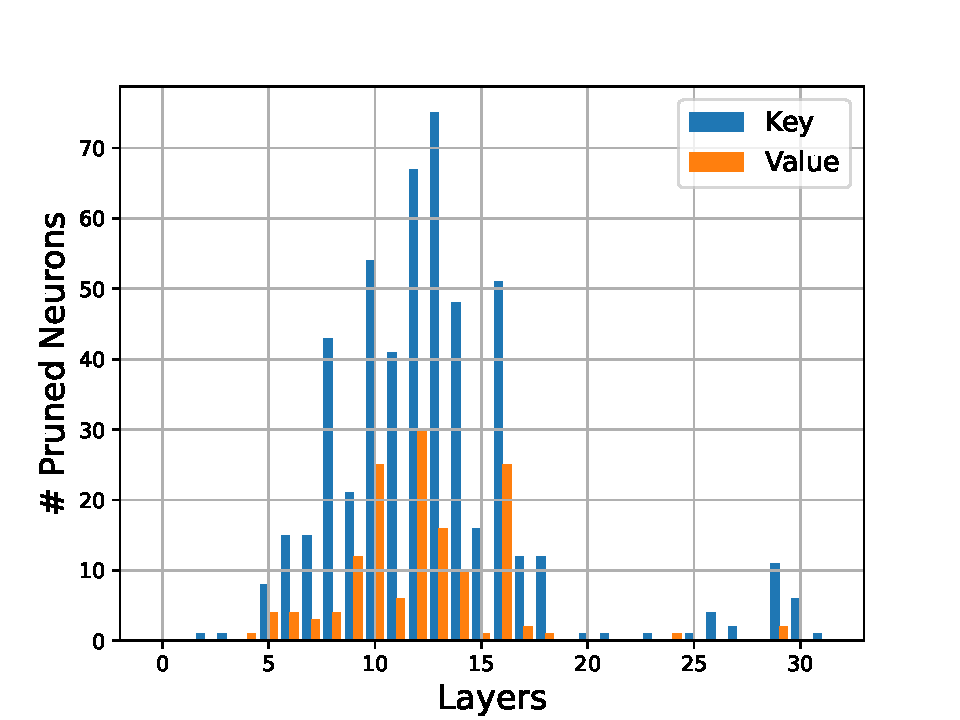
\includegraphics[width=\textwidth]{images/llama3_8b_hotpot.pdf}
        \caption{LLama3-8B}
    \end{subfigure}%
    ~ 
    \begin{subfigure}[t]{0.45\textwidth}
        \centering
        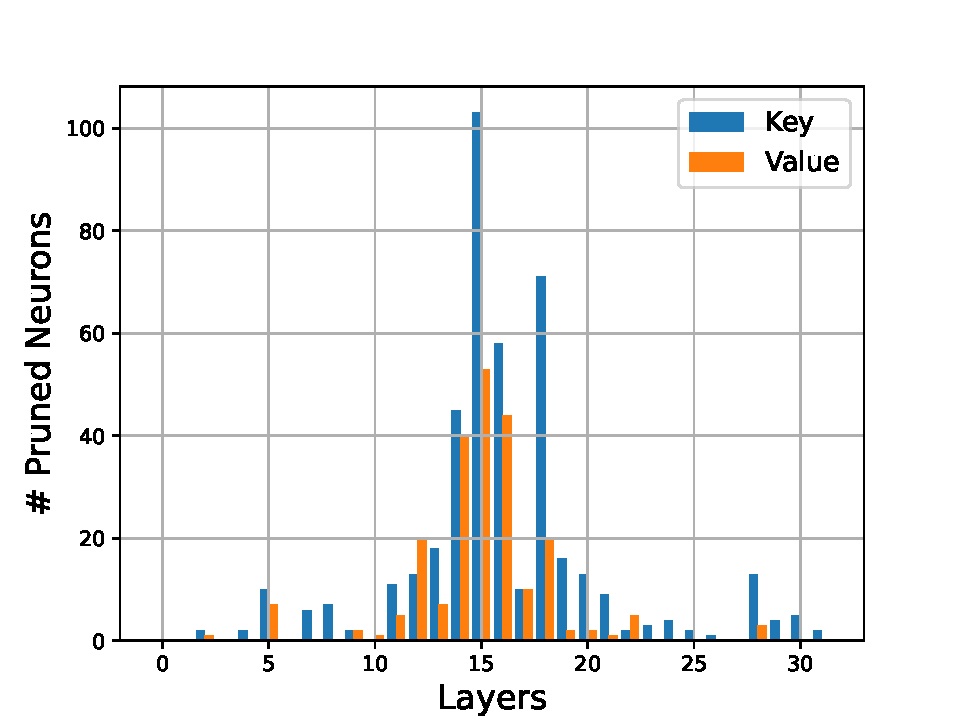
\includegraphics[width=\textwidth]{images/mistral_7b_hotpot.pdf}
        \caption{Mistral-7B}
    \end{subfigure}
    % \vspace{-1em}
    \caption{Distribution of the pruned neurons across different layers on the SQuAD dataset. }
    % \vspace{-1em}
    \label{fig:neurons_p}
\end{figure*}










\subsection{Experiment Setup}

% \textbf{Dataset.}
\textbf{Model and Dataset} We evaluate our approach on the model of LLama3-8B \cite{touvron2023llama}, Mistral-7B-Instruct-V3.0 \cite{jiang2023mistral} and Phi-3.5-mini-
instruct (3.8B) \cite{abdin2024phi3technicalreporthighly}.
By default, We experiment with $N=8$ for neural attribution and prune with $p=0.5$ ($0.5\%$ neurons).
% The learned mask from feature attribution is applied on all testing prompts. 
We evaluate with the question answering datasets of SQuAD \cite{rajpurkar2016squad} and HotpotQA \cite{yang2018hotpotqa},
% In preparing these datasets for indirect prompt inject 
using the splits directly processed by \citet{abdelnabi2024you},
% Specifically, in preparing the question-answering datasets for indirect prompt injection attack, \cite{abdelnabi2024you} 
Specifically, \citet{abdelnabi2024you} randomly injects instructions into the beginning, middle, and ending of the context of each prompt. 
% Compare with related detection-based approaches \cite{} approaches 
% Our approach focuses on the LLM's ability to distinguish between data and instructions, making it applicable to problems beyond defense against third-party injections.
% Specifically, 
We also explore a practical scenario of dialogue summarization with the WildChat \cite{zhao2024wildchat} dataset.
For this task, the model is attacked if it answers the question raised by users in the dialogue, instead of summarizing the dialogue interactions.
We use the same split as in \cite{abdelnabi2024you}. 
Initial experiments show that the models are rarely attacked with plain dialogues. 
Thus, to increase the difficulty, 
we insert \textit{"You should primarily focus on this question"} as part of the user instruction to the AI assistant that appeared in the dialogue. 
For each dataset, we randomly select  8 samples from a pool of ~400 prompts that are not overlapped with the testing data. 
The results are reported over 3 trials.
Please refer to Appendix \ref{app: details} for more details on baselines and metrics definitions.
Note that our \textit{CachePrune} is complementary to the existing baselines, since our approach does not modify the prompt formatting or require additional test-time overheads for response processing.


% \noindent\textbf{Model}

\
% \begin{figure}[t!] 
%     \centering
%     \begin{subfigure}[t]{0.24\textwidth}
%         \centering
%         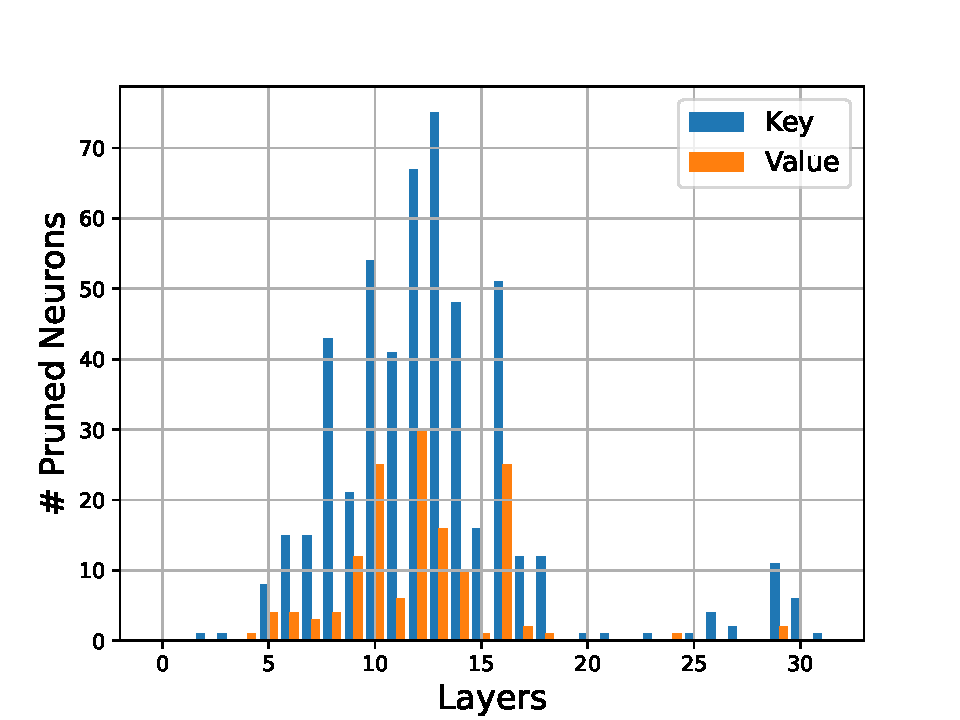
\includegraphics[width=\textwidth]{images/llama3_8b_hotpot.pdf}
%         \caption{LLama3-8B}
%     \end{subfigure}%
%     ~ 
%     \begin{subfigure}[t]{0.24\textwidth}
%         \centering
%         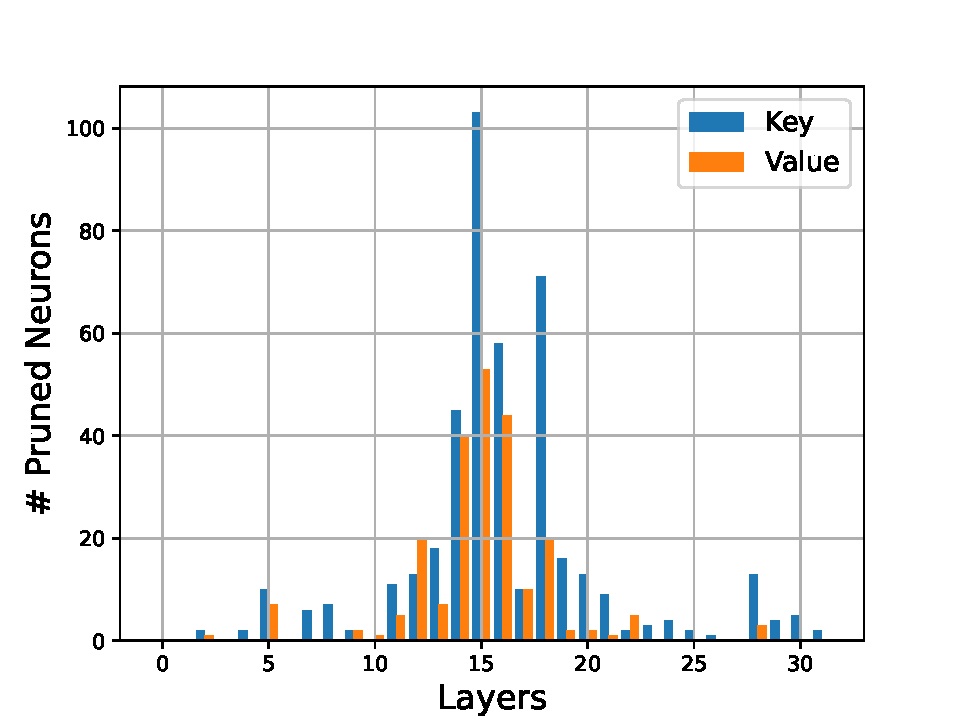
\includegraphics[width=\textwidth]{images/mistral_7b_hotpot.pdf}
%         \caption{Mistral-7B}
%     \end{subfigure}
    
%     \caption{Distribution of the pruned neurons across different layers on the SQuAD dataset.}
%     \label{fig:neurons}
% \end{figure}




% \begin{itemize}
%     \item \textit{Vanilla}: Query the LLM with the original prompt without any defense technique. We share the prompt templates in Appendix \ref{sec:prompt}.
%     \item \textit{Delimiting}: Adding special characters at the start and end of the context.
%     \item \textit{Datamarking}: Replace every space in the context with a special character \^, so that the context looks different from the user-specified instruction by the LLM.
%     \item \textit{Encode$\_$Base64}. This shares a similar motivation as Datamarking. The context is encoded into Base64 while the other text spans are provided with plain text. The LLM is required to decode the context to natural language. 
% \end{itemize}

% Our \textit{CachePrune} is implemented based on Vanilla. 

% We can conjure that approaches like Datamarking and Encode$\_$Base64 could potentially interfere with the LLMs' ability to understand the context, especially if the context is modified with special formatting.

% Our \textit{CachePrune} is actually complementary to these approaches since our approach does not modify the prompt.







% \begin{table*}
%     \centering
%     \caption{Terminologies in SQL and ...}
%     \label{tab:my_label}
%     \begin{tabularx}{0.5\textwidth}{X|X}
%     \toprule
%     \textbf{SQL} & \textbf{MONGODB} \\
%     \midrule
%     Database & Database \\
%     Table & Collection \\
%     Row & Document \\
%     Column & Field \\
%     Primary key (specify any unique column or column combination as primary key) & Primary key (the primary key is automatically set to the \_id field in MongoDB)\\
%     blah blah & blah blah \\
%     \bottomrule
%     \end{tabularx}
    
% \end{table*}







% \begin{table}[t]
% % \begin{wraptable}{r}{0.6\textwidth}
% \centering
% \small
% \begin{tabular}{l | c c c}
% \toprule
%   & \textbf{ASR} $\downarrow$ & \textbf{F1 (clean)} $\uparrow$ & \textbf{F1 (attack)} $\uparrow$ \\
% \midrule
% {k=1}    & 7.44 $\pm$ 0.22 & 28.68 $\pm$ 0.30 & 22.84 $\pm$ 0.49 \\
% {k=2}  & 5.57 $\pm$ 0.30 & 26.03 $\pm$ 0.28 & 22.47 $\pm$ 0.37 \\
% {k=4}    & 10.77 $\pm$ 0.45& 24.71 $\pm$ 0.37 & 19.29 $\pm$ 0.33 \\
% $\mathcal L^{attr}_{full}$     & 14.81 $\pm$ 0.59 & 25.63 $\pm$ 0.39 & 19.78 $\pm$  0.55\\
% \bottomrule
% \end{tabular}
% \vspace{-1em}
% \caption{Performance of LLama3-8b on SQuAD with different  $k$. $\mathcal L^{attr}_{full}$ means we attribute with all the tokens in the response.}
% \label{tb:lr}
% \vspace{-1em}
% \end{table}


% \begin{table}[t]
% % \begin{wraptable}{r}{0.6\textwidth}
% \centering
% \small
% \begin{tabular}{l | c c c}
% \toprule
%   & \textbf{ASR} $\downarrow$ & \textbf{F1 (clean)} $\uparrow$ & \textbf{F1 (attack)} $\uparrow$ \\
% \midrule
% {$\alpha$=1.5}    & 6.40 $\pm$ 0.32 & 26.71 $\pm$ 0.53 & 20.22 $\pm$ 0.56 \\
% {$\alpha$=1.0}  & 7.44 $\pm$ 0.22 & 28.68 $\pm$ 0.30 & 22.84 $\pm$ 0.49 \\
% {$\alpha$=0.5}    & 10.77 $\pm$ 0.61 & 28.33 $\pm$ 0.40 & 21.29 $\pm$ 0.61\\
% {$\alpha$=0.3}     & 13.50 $\pm$ 0.70 & 28.91 $\pm$ 0.37 & 21.78 $\pm$ 0.43\\
% \bottomrule
% \end{tabular}
% \vspace{-1em}
% \caption{Performance of LLama3-8b on SQuAD with differen values of $\alpha$. 
% % $\mathcal L^{attr}_{full}$ means we attribute with all the tokens in the response.
% }
% \label{tb:mask}
% \vspace{-1em}
% \end{table}


% \begin{table}[t]
% % \begin{wraptable}{r}{0.6\textwidth}
% \centering
% \small

%  \begin{minipage}[b]{\linewidth}
% \resizebox{\linewidth}{!}{
% \begin{tabular}{l | c c c}
% \toprule
%   & \textbf{ASR} $\downarrow$ & \textbf{F1 (clean)} $\uparrow$ & \textbf{F1 (attack)} $\uparrow$ \\
% \midrule
% Vanilla Code               & 17.5  & 29.01  & 22.56 \\
% Code $\rightarrow$ Code    & 1.77 $\pm$ 0.13 & 31.38 $\pm$1.22 & 24.30 $\pm$ 0.65 \\
% Text $\rightarrow$ Code  & 3.20 $\pm$ 0.53 & 32.20 $\pm$ 1.08 & 25.87 $\pm$ 0.82 \\
% \hline
% \hline
% Vanilla Text               & 45.15  & 26.96 & 12.35 \\
% Text $\rightarrow$ Text    & 9.23 $\pm$ 0.39 & 27.33 $\pm$ 1.45 &  21.39 $\pm$ 1.13 \\
% Code $\rightarrow$ Text     & 16.9 $\pm$ 1.25 & 26.57 $\pm$ 0.76 & 20.21 $\pm$0.42 \\
% \bottomrule
% \end{tabular}
% }
% \vspace{-1em}
% \caption{
% Transferring the mask from feature attribution between code-based and text-based injection. Learning a mask from prompt with code/text injections and apply on data with text/code injections. 
% % Our learnt mask is transferrable between different kind of injection tasks.
% % Performance of LLama3-8b on SQuAD with differen values of $\alpha$. 
% % $\mathcal L^{attr}_{full}$ means we attribute with all the tokens in the response.
% }
% \label{tb:transfer}
% \end{minipage}

% \vspace{-2em}
% \end{table}










% \begin{table}[t]
% % \begin{wraptable}{r}{0.6\textwidth}
% \centering
% \small
%  \begin{minipage}[b]{\linewidth}
% \resizebox{\linewidth}{!}{

% \begin{tabular}{l | c c c c}
% \toprule
%     & \textbf{w/ $\Phi$} & \textbf{ASR} & \textbf{F1 (clean)} & \textbf{F1 (attack)} \\
% \midrule
%  \multirow{2}{*}{$\alpha$=1.5} & Y & 6.40 $\pm$ 0.32 & 26.71 $\pm$ 0.53 & 20.22 $\pm$ 0.56 \\
%   & N& 6.40 $\pm$ 0.32 & 26.71 $\pm$ 0.53 & 20.22 $\pm$ 0.56 \\
% % {$\alpha$=1.0}  & 7.44 $\pm$ 0.22 & 28.68 $\pm$ 0.30 & 22.84 $\pm$ 0.49 \\
% % {$\alpha$=0.5}    & 10.77 $\pm$ 0.61 & 28.33 $\pm$ 0.40 & 21.29 $\pm$ 0.61\\
% % {$\alpha$=0.3}     & 13.50 $\pm$ 0.70 & 28.91 $\pm$ 0.37 & 21.78 $\pm$ 0.43\\
% \bottomrule
% \end{tabular}
% \vspace{-1em}
% \caption{Performance of LLama3-8b on SQuAD with differen values of $\alpha$. 
% % $\mathcal L^{attr}_{full}$ means we attribute with all the tokens in the response.
% }
% }
% \label{tb:phi}
% \end{minipage}
% \vspace{-1em}
% \end{table}

\begin{figure*}[htbp]
% \vspace{-2mm}
  \centering
  \begin{subfigure}[t]{0.32\textwidth}
    \centering
    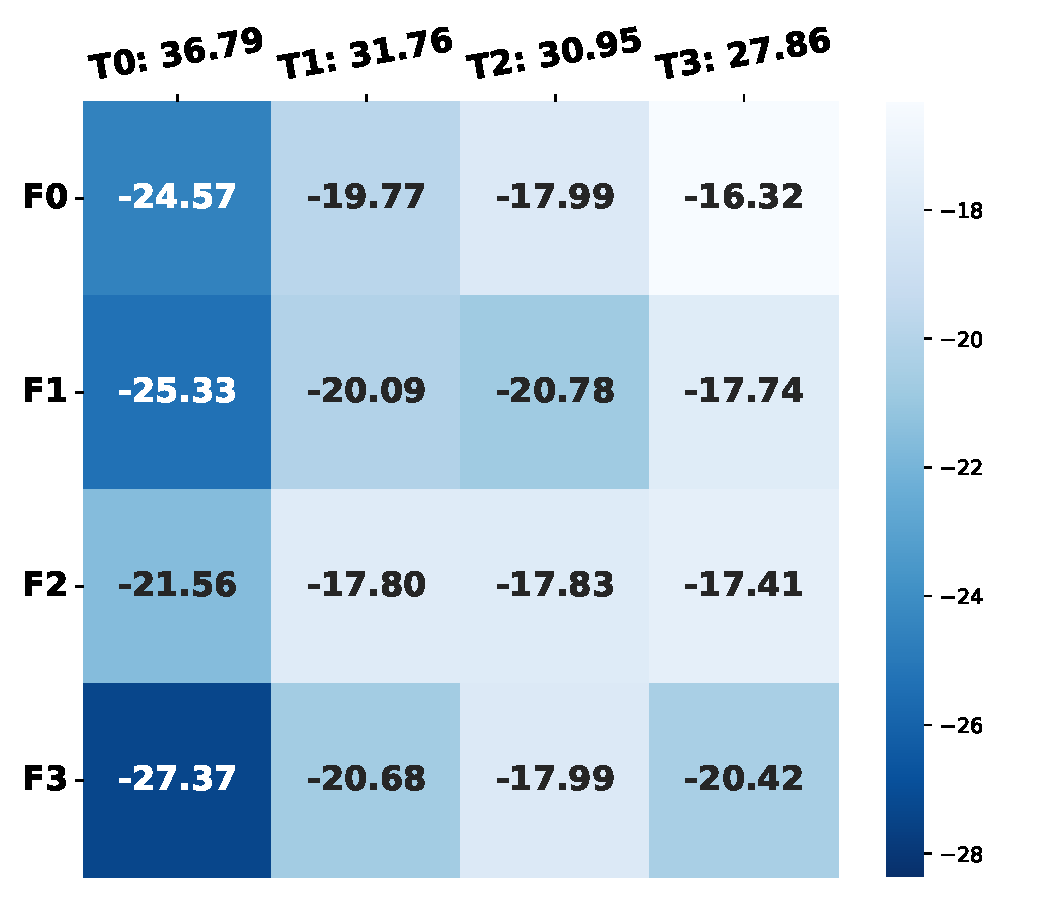
\includegraphics[width=\textwidth]{images/asr.pdf}
    \caption{ASR}
    \label{fig:subfig1}
  \end{subfigure}
  \hfill
  \begin{subfigure}[t]{0.32\textwidth}
    \centering
    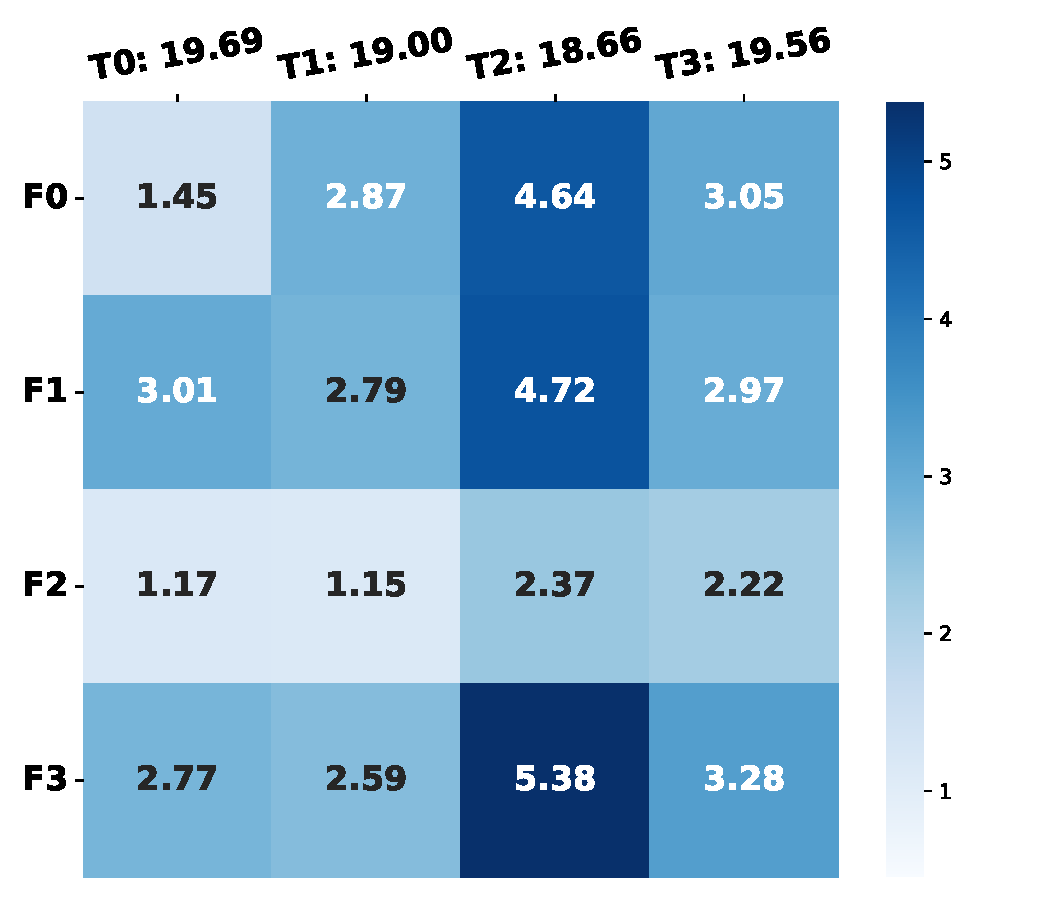
\includegraphics[width=\textwidth]{images/f1_attack.pdf}
    \caption{F1 (attack)}
    \label{fig:subfig2}
  \end{subfigure}
  \hfill
  \begin{subfigure}[t]{0.32\textwidth}
    \centering
    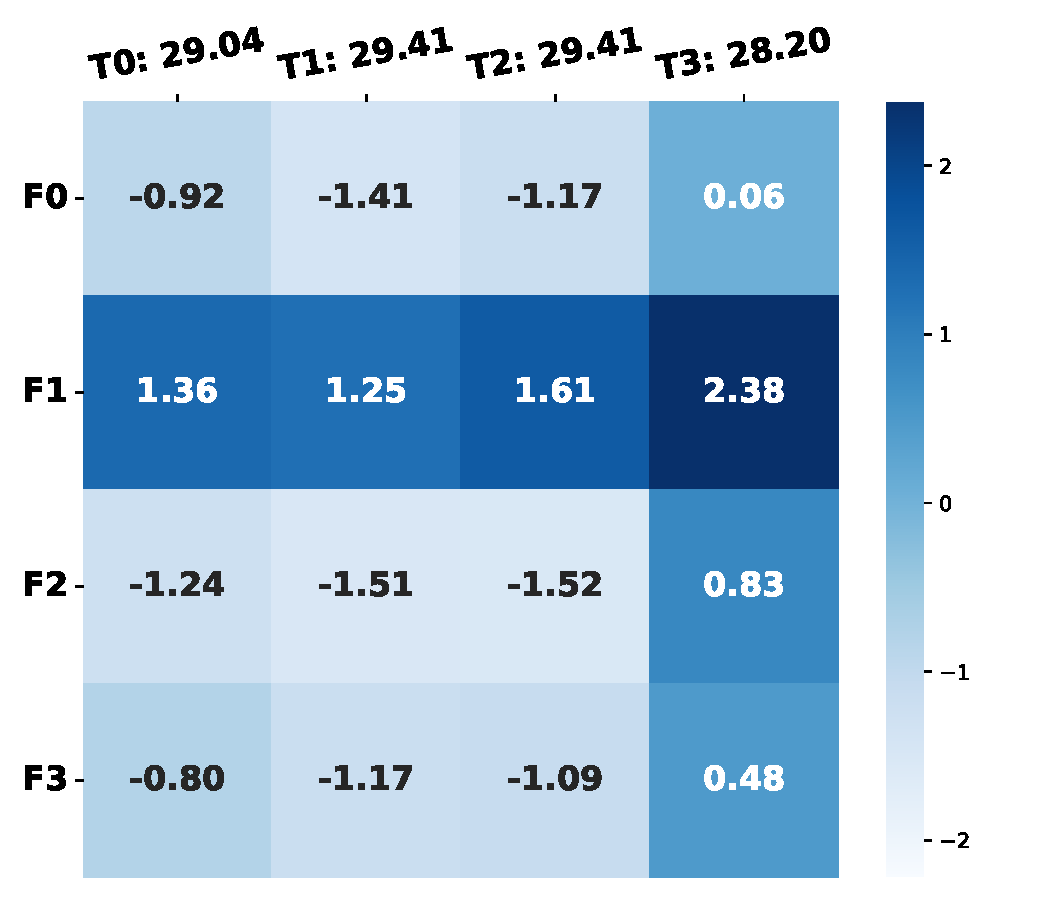
\includegraphics[width=\textwidth]{images/f1_clean-2.pdf}
    \caption{f1 (clean)}
    \label{fig:subfig3}
  \end{subfigure}
  \vspace{-1mm}
  \caption{Transferring the learnt mask between prompts with different attacks instructions on SQUaD with LLama3-8b. 0-3 corrsponds to 4 different attacks instructions described in Appendix \ref{app: trans}. Each value in the matrix can be formatted with $[Fi, Tj: s]$. $i,j$ means using the mask learn from prompts attacted by $i$ to pruning KV cache from prompts attacked by $j$.  $s$ is the vanilla baseline on $j$ without any defense. The value of $[Fi, Tj: s]$ means the gain in ASR or F1 compared to $s$. For example, $[F0, T3: 27.86]$ in (a) means the ASR of applying the mask learnt from attack $0$ to attack $1$ is $27.86+(-16.32)=11.54$. We have dark color highlight more negative gain for ASR and more positive gain for F1. Therefore, if the learnt masks are not transferrable between different attacks, we would expect three diagonal matrix in color. However, we can see that the darkest color does not necessrily appear  in the diagonal. Therefore, our learn mask for pruning is transferrable between different attacks.}
  \label{fig:three_in_a_row}
  \vspace{-3mm}
\end{figure*}



\begin{figure}[t!] 

        \centering
        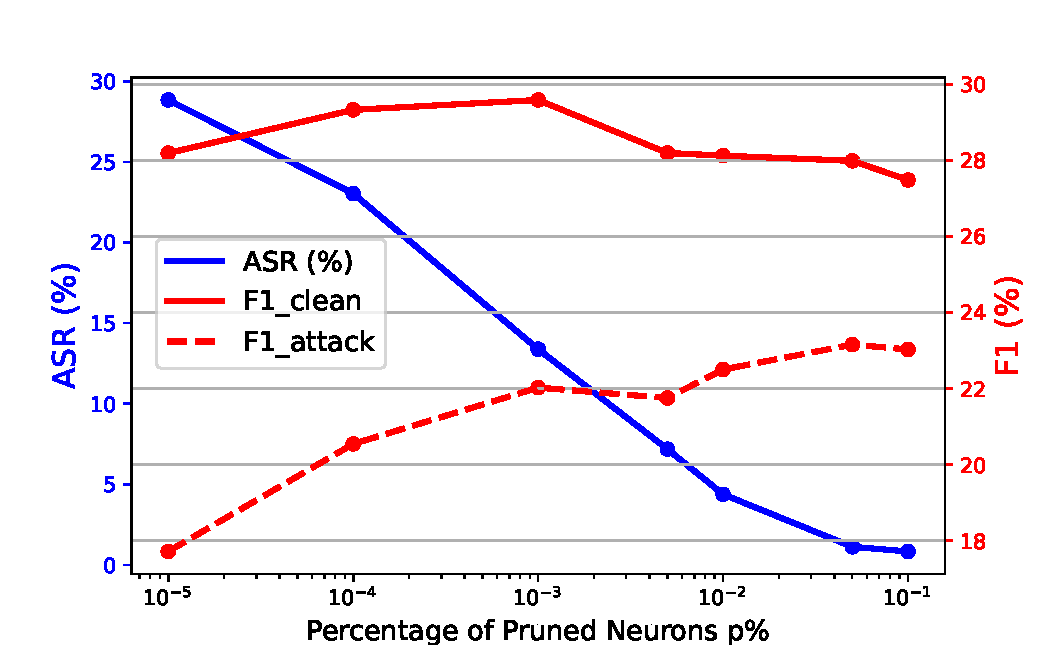
\includegraphics[width=0.42\textwidth]{images/percentage_llama38b_h.pdf}
        % \caption{LLama3-8B}

    % \vspace{-1em}
    \caption{Performance of LLama3-8 on SQuAD with different percentage of pruned neurons $p$.}
    % \vspace{-2em}
    \label{fig:neurons}
    \vspace{-1em}
\end{figure}



% \vspace{-4mm}
\subsection{Result Analysis}

We summarize the results in Table \ref{tb: fdu}. 
Our proposed \textit{CachePrune} significantly reduces the Attack Success Rate (ASR) as compared to the baselines, while maintaining the response quality in following user instructions.
% in addressing the user-specified instructions.

Specifically, the ASR with our proposed \textit{CachePrune} can be several times lower than \textit{Vanilla}, \textit{Delimiting}, and \textit{Datamarking}. The \textit{Encode$\_$Base64} yields ASR that is comparable to \textit{CachePrune}, but at the expense of very low F1 scores. 
We reckon that this is because the modification on context with \textit{Encode$\_$Base64} is too complex for our LLMs, resulting in the model understanding the context.
This highlights a deficiency of defending with prompt engineering, \emph{i.e.}, the manually designed complex marking on the input context may increase the difficulty for the LLM to comprehend the context information. 
On the contrary, our approach leverages the LLMs' discretion on the difference between data and instruction, instead of relying on complex human engineering. Additionally, we can find that the score of F1 (attack) is generally lower than F1 (clean), suggesting that responding to the injected instructions could limit the LLMs' ability to solve the user-specified ones.
% Our \textit{CachePrune} yields the highest F1 (attack) of our  is generally 





In Figure \ref{fig:neurons_p}, we plot the distribution of pruned neurons across layers. It can be observed that,
% \begin{itemize}
%     \item The neurons pruned concentrate in the middle layers of the LLM. This is aligned with previous studies, \emph{e.g.}, \citet{huang2024learn}, showing that the middle layers are more capable of capturing abstract and complex concepts.
%     \item Additionally, it is interesting to find that there are generally more key neurons being pruned than value neurons. Since the key neurons controls the self-attention in Transformer, this suggests that our approach works by intervening how a newly generated token attends to tokens from context, so that it treats these tokens as data instead of instruction. In the meanwhile, the less pruning on the value shows that the pruning is preserving the encoded content (value) of the input context, thus maintaining the quality of clean responses that rely on this contextual knowledge.
% \end{itemize}
the neurons pruned concentrate in the middle layers of the LLM.
This is aligned with previous studies, \emph{e.g.}, \citet{huang2024learn}, showing that the middle layers are more capable of capturing abstract and complex concepts.
% Additionally, it is interesting to find that there are more key neurons being pruned in layers of LLama3-8b, indicating that the LLama model is trained to perceive instructions with the key vectors. 
% In comparison, the Mistral model is more balanced with keys and values in distinguishing between the concepts of data vs. instructions.
Additionally, it is interesting to find that there are generally more key neurons being pruned than value neurons. Since the key neurons controls the self-attention in Transformer \cite{geva2021transformer}, this suggests that our approach works by intervening how a newly generated token attends to tokens from context, so that it treats context tokens as data instead of instructions. 
In the meanwhile, the less pruning on the value shows that the pruning is preserving the encoded content of the input context, thus maintaining the quality of clean responses that rely on the context knowledge.
In Figure \ref{fig:neurons}, we plot the model performance with the prune ratio $p$. 
It can be observed that the pruning not necessarily decrease the F1 (clean). 
This could because applying the pruning masking ove the context informs the LLM of the prompt structure (context vs instruction).

In Table \ref{tb:lr}, we list the performance of LLama3-8B on  SQuAD, with different values of $k$.
% , where $\mathcal L^{attr}_{full}$ denotes $k$ taking its largest value by attribution with all the response tokens. 
This suggests that earlier tokens in the response are more indicative of the model’s preference between poisoned and clean outputs.
% the generation path, \emph{i.e.}, either treat the input context as pure data or indications of the instruction following irrespective of the user-specified prompt structure.
Table \ref{tb:mask} shows the performance with the different masking parameter $\alpha$. 
With $\alpha$ getting larger, the model is increasingly treating the context as instructions, which is demonstrated by a larger ASR. It shows that our identified neurons are indeed reflecting the model's implicit criteria on the distinction between  data and instruction.
%, with lower ASR corresponding to larger degree of masking ($\alpha\uparrow$).
In Table \ref{tb:transfer}, we show with SQUaD that the pruning mask learnt from text/code-based injection can be effectively transferred to defend code/text-based injection.
We inject in SQuAD context with code-based injection task from \citet{codealpaca} and text-based injection task from \citet{ji2023beavertails}.
In Figure \ref{fig:three_in_a_row}, we also show that our learnt pruning mask is transferrable across different attack instructions. Details of the experimental setup are provided in Appendix~\ref{app: trans}.